\pagestyle{fancy}
\lhead{}
\renewcommand{\headrulewidth}{0pt}
\setlength{\headheight}{14pt}

\chapter{Introduction}
\label{chapter:Intro}

Especially in rural areas, today's world of clubs is dominated by small and medium size organisations. Based on my experience, these clubs are mostly managed using outdated techniques and their communication channels are mostly handled through existing social networks, electronic or non-electronic mail. This is due to the fact that most of the members and management boards of the societies are either not familiar enough with the complexity of the few modern club management solutions, do not know of their existence or can't see the implications of using them.

\emph{myVerein} is trying to solve these problems and provide a comprehensive and intuitive solutions for small and medium size clubs. This solution should use the benefits of the recent developments of the IT industry and the principles of cloud and mobility solutions to create the club management solution of the 21\textsuperscript{st} century. 

In the following chapters the process of planning and designing as well as the execution is going to be discussed. 

\section{Market analysis}
\label{sec:MarketAnalysis}

A common principle in todays business is analysing all comparable products and solutions, that are used by potential customers. These solutions might not even be designed for that purpose, but could be misused by the user, because they fit their need.

The most important part is the identification of the mistakes the competitors made and learn from their behaviour \cite{Hunter:2015aa}. From these findings, it is possible and important to draw parallels and use them to \enquote{model what is working for your competition and [...] not copy your competition directly} \cite{Hunter:2015aa}. 

There exists several ways of identifying and monitoring competitors. When talking to potential customer, it is possible to get a closer look at their current solutions \cite{Philips:2015aa}. Another possible way is to use web searches to try and find solution targeted at your problem. With the help of a search engine it is also possible to get a first look on the presentation and marketing concepts of the identified rivals \cite{Philips:2015aa}. Of course there are additional steps available, including gathering information within social media platforms, at trade conferences or email newsletter \cite{Dahl:2011aa}. 

Within this section the competing services that have been found and analysed in preparation of this work are going to be presented. This analysis was possible thanks to the help and feedback of administrators from the \emph{Freiwillige Feuerwehr Lohr} and \emph{Melomania Helmstadt}. Only one direct competitor could be identified. This product is created by \emph{Buhl Data Service}. Nevertheless a mix of different services is combined by the users, since there is no comprehensive solution available for them. The presented concept and implementation in the upcoming chapters is based on these findings.

\subsection{Buhl Data Service}

The \emph{Buhl Data Service} company offers several solutions for the private and small to medium size business sector. Among them are applications used for the creation of tax statements and private banking. All solutions are intended to be used on the German market, since they cover country specific topics \cite{Buhl:2015aa}. Besides the above mentioned products \emph{Buhl Data Service} is also offering an application called \enquote{WISO Mein Verein}, whose purpose is the managing of members of a society as well as several other related tasks.

\emph{WISO Mein Verein} was initially designed to only be used by a single user at once. Later the developer introduced a team edition, which offered the ability to upload the database backing the application to a centralised repository, but while the data was modified, it is still not possible for a second user to access the data. In general this process of lock - modify - unlock is very unintuitive and lacks of transparency. This process therefore reduces the usability dramatically, especially for administration without a technical background.

The functionalities provided by the application are very rich. They range from simply listing all members, to the creation of automated debit transfers as well as storing and populating templates for non-electronic newsletter. The suite itself is a very mature product, only its graphical user interface and missing cross platform functionalities are not completely meeting today's standards \cite{Buhl:2015ab}. 

During this project the company launched the public beta of a newly created online social network, targeting member and administrators of clubs. The service is integrated into the \emph{WISO Mein Verein} environment and called \emph{Mein Verein}. An administrator has the possibility to import the data from his \emph{WISO Mein Verein} suite and invite all users to use the social network. 

The network is accessible through a web portal and an Android and iOS app. The portal covers all expected functionalities of a modern social network targeted at members of clubs, including messaging, calendar functions and the ability to search, join and create societies. 

Unfortunately this service was very new, and therefore the time did not permit the extensive testing of this portal. Some question did arise while research on this product. It was unclear how well the process of managing the club is integrated in the web portal, specifically speaking if all functionalities known from \emph{WISO Mein Verein} are available through \emph{Mein Verein} or if the administration needs to maintain two separated data sets, that might become inconsistent. 

Both solutions do not share a common pricing scheme. \emph{WISO Mein Verein} is charged separately yearly, starting at 69,99 Euro for the single user version and 139,95 Euro for the team version \cite{Buhl:2015ab}. On the other hand the usage of the web portal \emph{Mein Verein} is completely free of charge and advertisement free. This leads to the question how \emph{Buhl Data Service} is planing monetising that product. Since the portal is handling private user data and is also holding private bank details, in case it is connected to the \emph{WISO Mein Verein} suite, it is crucial that these data is not shared with a third party.

\subsection{In-comprehensive solution}

A comprehensive solution covering both, managing a club as well as creating a unified communication channel is only partly realised through the \emph{Mein Verein} portal. On top of that the network just recently left it's beta testing phase and is therefore a very young and probably unknown application. Concluding a lot of users as well as administrators started trying to create their own way of handling this problem. 

While talking to several club members of different societies as well as my own experience a couple of existing social network and messaging application are misused to connect the user and informing them about news concerning their club. 

One very popular option is the usage of hidden \emph{Facebook} groups, creating a broadcasting channel for administrators as well as user. Depending on the size of these groups, the personal notification system of the user's \emph{Facebook} may be flooded by unrelated and therefore uninteresting information. On top of that many user do not provide their actual personal information or aren't part of the network because of privacy reasons and therefore the user register created by these groups is incomplete, especially if the administrator is trying to communicate using traditional channels as well. 

Another possibility is the usage of instant messaging services like \emph{WhatsApp}. They are providing group messaging features. Unfortunately every user receives a notification for each message send through the group. Especially if there is a vivid discussion a user is not part of, the amount of received notification might get annoying. This system also does not provide any user or event management at all. So this needs to be done either through a separate channel, or the users need to manually maintain their calendar.

In total all these products have a unique use-case, but do not offer any comprehensive solution to the problem of managing a club and unifying its communication. Nevertheless there is a reason that these products are very popular among users. Therefore the positive aspects should be closely examined and adopted, while resolving the shown problems.

\section{User analysis}
\label{sec:UserAnalysis}

During the creation of a product it is crucial to meet the requirements of the user. Especially during the creation of an user interface this holds true. In general a user is not going to spend much time on searching functionalities, which means he might be less satisfied with the product and consequentially use it less frequent, even though it implements all necessary requirements \cite{Frank:2013aa}. Therefore every functionality needs to be arranged logically and specifically tailored to the target audience.

This process is called usability engineering and focuses on guiding through the necessary steps resulting into a satisfying user experience \cite{Nielsen:1993aa}. The most important part is \enquote{the process of identifying users’ needs to ensure a product can achieve specific goals effectively and efficiently, which results in overall satisfaction and success} \cite{Frank:2013aa}.

The importance of usability engineering can also be seen in the fact, that the \gls{ISO} is covering this topic as part of the ISO 9241 standard. The author is referring to section 210 of the standard, which is labelled \enquote{Human-centred design for interactive systems}.It is describing the general development cycle of an user interface, where the user analysis itself is playing an important part \cite[p. 13]{Gulzow:2015aa}.

The usability engineering describes 2 major kinds of methods to analyse an user: analytical and empiric \cite[p. 20]{Gulzow:2015aa}. Within an analytical approach the developer is trying to see things from a user's perspective, where empiric methods involve the user directly. 

For this project the \emph{Persona} method was used to perform a user analysis. Personas are several relevant users, who are described by their archetypal properties. Additionally their behaviour and objectives are presented \cite[p. 30]{Gulzow:2015aa} These findings are mainly based on personal experience, as well as information received by different club administrators. The different personas are presented ordered from the most to the least relevant one.

\subsubsection{Jacob - 41}
\label{sec:Jacob}

Jacob is father of two children. He lives in a small house with his family in the outskirts of a small German town. Besides his work at a global oriented medium sized technology company, he is a volunteering member at the local sports club. Generally speaking he is technology affine, but not an expert. His job is managing all members of the club. This includes the listing of all active and passive members, as well as ensuring that everyone paid their membership fees. Additionally he has the responsibility to invite all members to events organised by the club. 

The utilities Jacob is using to do his job at the club include an Excel sheet with all names and contact details, as well as a Word template for his invitations for several events. Recently he created an email distribution list to save the money he always spend on mailing the paper letters. Besides a handful older members everyone is receiving these emails. Nevertheless the constantly changing club structure and contact details are hard to manage and he spends a lot of time updating his member list.

\subsubsection{Marie - 21}
Marie is a student and recently moved out of her parent's house. She is an active soccer player since nearly 10 years at the sport club. Unfortunately she often misses special events organised by her club, because in the past she barely paid attention for the club mail, handled by her parents. Since she is receiving emails from her club on her smartphone she regularly updates her calendar according to the events, but slowly gets annoyed by the amount of data she has to organise besides her studies.

On top of that she is part of a \emph{WhatsApp} group dedicated to her team where all kinds of topics are discussed, ranging from the last party to the next game. On top of that a soccer group dedicated to her club was created on \emph{Facebook}, where additional information are shared.

Since she just lately moved she is trying to change her contact details registered at the club. Unfortunately after asking her coach and the head of the club to change the information she is currently waiting for a conformation from Jacob about the successful change. All in all she is not very satisfied with the current infrastructure and possibilities offered by the club.

\subsubsection{Karl - 58}
Karl is a farther of 2 and grandfather of 5. He had lived together with his wife in the same house for nearly 30 years. Even longer he has been a part of the local sports club. Because of his age he is not as active as he used to be, but he helps everywhere he can. The electrician plays an important part in maintaining the club house and supporting teams during their game days.

Even though he owns a PC, which was a present from his children, he is not very confident using it. Therefore he does not receive any information through email, but through traditional non-electronic mail, as well as through personal contact with the responsible parties.  

\chapter{Unique selling point}
\label{chapter:SellingPoint}

The result of the market analysis in section \vref{sec:MarketAnalysis} as well as the user analysis in section \vref{sec:UserAnalysis} lead to the conclusion that there is the need for a comprehensive solution. Using these findings, the key points of the application can now be derived. 

The first and most important point of the application is to reduce the workload on the person managing the members of the club as well as advertising events, described as Jacob in section \vref{sec:Jacob}. Since this person is already spending at lot of his time on keeping the club running, mostly free of any charge, he should perform his work as efficient as possible. This should also include the possibility to delegate work to other people, e.g. every user could be responsible to keep his contact information up-to-date, without the need of the administrator being actively involved.

The second point of the application is reducing the personal organisation overhead for a single user. Specifically talking a user should be automatic reminded of upcoming events and he should have an easy way of checking a personalised, up to date schedule of her club related events.

Lastly the group pressure on individuals to join one or multiple social networks or applications should be removed, by providing a safe and trustfully environment. On top of that people that are not able or do not feel confident with using latest technology should not be forced into using it. In contrast a viable alternative should be offered to these users. 

These three points basically cover the main idea behind this project. Of course, several more key points could be concluded from the findings in chapter \vref{chapter:Intro}. Unfortunately these would push the boundaries of this project. Nevertheless they are briefly discussed in chapter \vref{chapter:OngoingWork}.

\chapter{Concept}
\label{chapter:Concept}
Within this chapter the initial thoughts, leading to the concept of the application, are described, respecting the findings from chapter \ref{chapter:Intro}. This chapter will present different approaches that could have been chosen to solve the problem. An evaluation of these possibilities, based on feasibility, necessity and user value is going to be provided later.

\section{Platform} % Mapping to deployment model/ER model/architectural overview
\label{sec:Platform}
Nowadays a solution can be created focusing on a wide area of devices and using several technologies supported by these platforms. In general, the workload increases with each platform, and/or technology that is included into the development process. Concluding a well balanced trade-off needs to be made when choosing platform and technology for a project.

The most conservative approach is developing a stand-alone desktop application. The interaction using mouse and keyboard is the most established one and possibly the only point of contact with modern \gls{IT} systems for non-technology oriented people. Nevertheless this platform and technology is concluding several negative aspects: A single platform needs to be chosen and every additional platform would include a massive amount of supplementary work, based on the assumption of not using cross platform technologies, like \emph{\Acrfull{WOCA}} or \emph{\Acrfull{WORA}}. On top of that the time spend online on mobile devices recently surpassed desktop application \cite{Murtagh:2014aa}, which reduces the importance of them. 

\begin{figure}[h]
	\centering
	\begin{subfigure}{.49\textwidth}
  		\centering
  		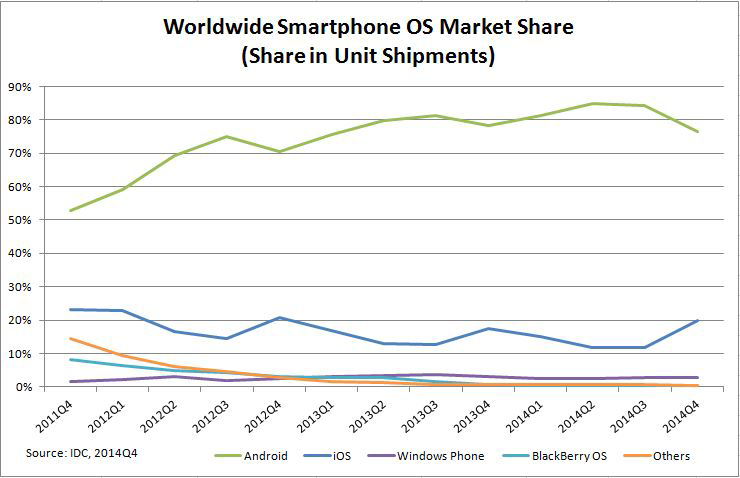
\includegraphics[width=0.98\linewidth]{./images/smartphone-os-market-share.png}
  		\caption{Operating Systems}
  		\label{fig:OSMarketShare}
	\end{subfigure}
	\begin{subfigure}{.49\textwidth}
  		\centering
  		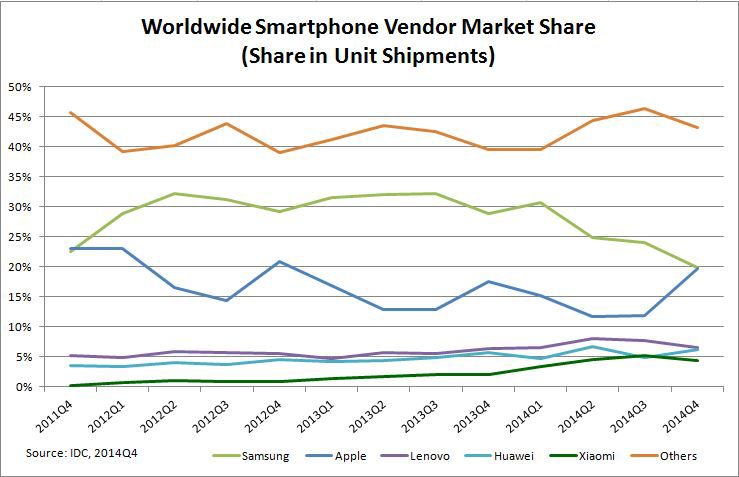
\includegraphics[width=0.98\linewidth]{./images/smartphone-vendor-market-share.png}
  		\caption{Vendors}
  		\label{fig:VendorMarketShare}
	\end{subfigure}
	\caption[Smartphone operating system's and vendor's market share, Q4 2014, retrieved from \cite{IDC:2015aa} and \cite{IDC:2015ab}]{Smartphone market share, Q4 2014}
	\label{fig:Shares}
\end{figure}
\nocite{IDC:2015aa, IDC:2015ab}

As shown in the last paragraph the importance of mobile applications rose tremendously within the last couple of years. Therefore it is essential to take this platform into consideration. When looking at the market shares of mobile \gls{OS}, shown in figure \vref{fig:OSMarketShare}, it seems obvious that an application should initially be developed for the \emph{Android} platform, since it got a market share of 76.6\% \cite{IDC:2015aa}. Later the development for \emph{iOS} (19.7\%) and \emph{Windows Phone} (2.8\%) might be considered \cite{IDC:2015aa}. But when looking at vendor market shares, shown in figure \vref{fig:VendorMarketShare}, this picture is not so obvious anymore. \emph{Apple}, the only vendor distributing devices with the \emph{iOS} \gls{OS}, has nearly the same market share as \emph{Samsung}, the biggest vendor of \emph{Android} running mobile devices \cite{IDC:2015ab}.

\begin{figure}[h]
	\centering
	\begin{subfigure}{.49\textwidth}
  		\centering
  		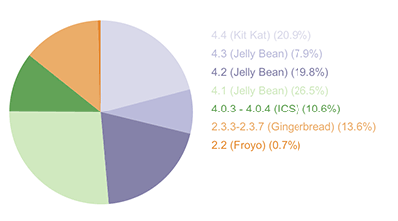
\includegraphics[width=0.98\linewidth]{./images/android-os.png}
  		\caption{Android}
  		\label{fig:AndroidOSFragmentation}
	\end{subfigure}
	\begin{subfigure}{.49\textwidth}
  		\centering
  		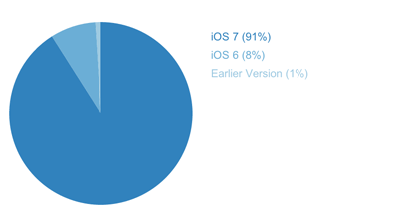
\includegraphics[width=0.98\linewidth]{./images/ios-os.png}
  		\caption{iOS}
  		\label{fig:iOSOSFragmentation}
	\end{subfigure}
	\caption[Mobile \gls{OS} fragmentation, retrieved from \cite{OpenSignal:2014aa}]{Mobile \gls{OS} fragmentation}
	\label{fig:MobileOSFragmentation}
\end{figure}
\nocite{OpenSignal:2014aa}

As already hinted, the \emph{Android} platform seems more fragmented than the \emph{iOS} eco-system. This is due to the fact that the \gls{OS} is distributed by several vendors, which create device with different specification. On top of that the support for the latest version of the \gls{OS} is not guaranteed, which not only leaves devices open for security vulnerabilities, but also increases the workload for the developer. As shown in figure \vref{fig:iOSOSFragmentation}, nearly 99\% of the \emph{iOS} devices were running the two latest versions of the \gls{OS} in 2014. In opposite to that, figure \ref{fig:AndroidOSFragmentation} shows that not even 50\% of the \emph{Android} devices were running the three latest revisions of the platform. This fragmentation is also reflected by figure \vref{fig:MobileScreenFragmentation}, which is showing all screen sizes of mobile devices running \emph{Android}, respectively \emph{iOS}, as of 2014.

\begin{figure}[h]
	\centering
	\begin{subfigure}{.49\textwidth}
  		\centering
  		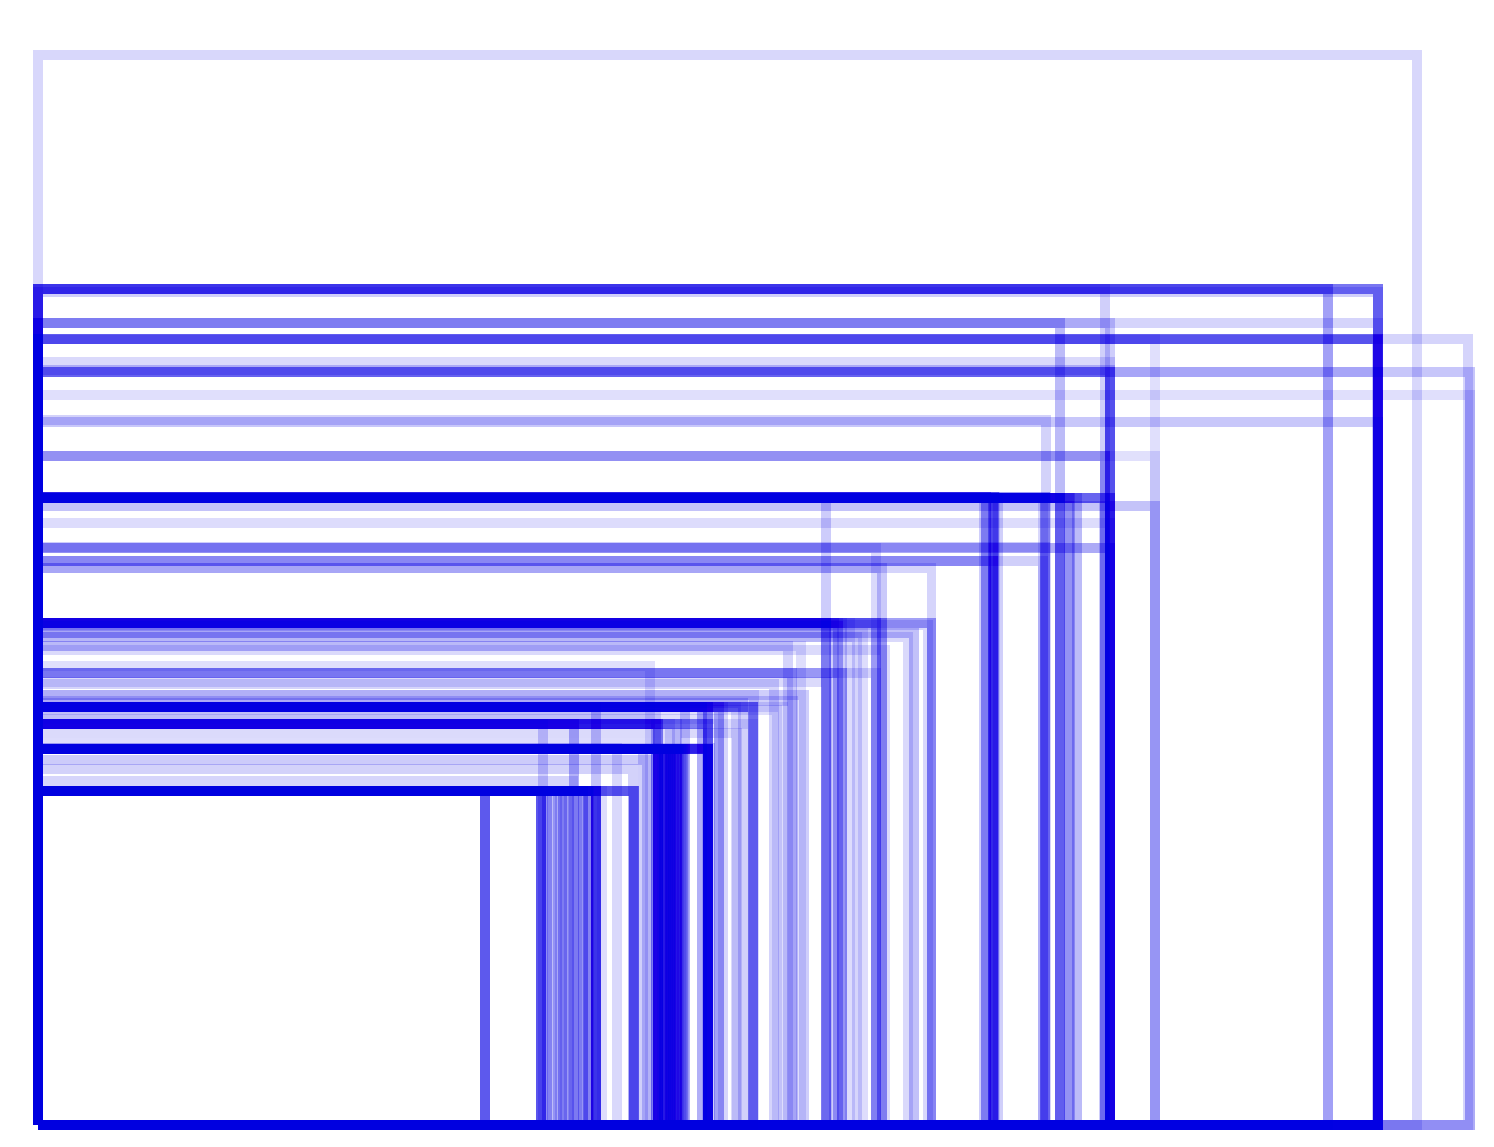
\includegraphics[width=0.98\linewidth]{./images/android-screen.png}
  		\caption{Android}
  		\label{fig:AndroidScreenFragmentation}
	\end{subfigure}
	\begin{subfigure}{.49\textwidth}
  		\centering
  		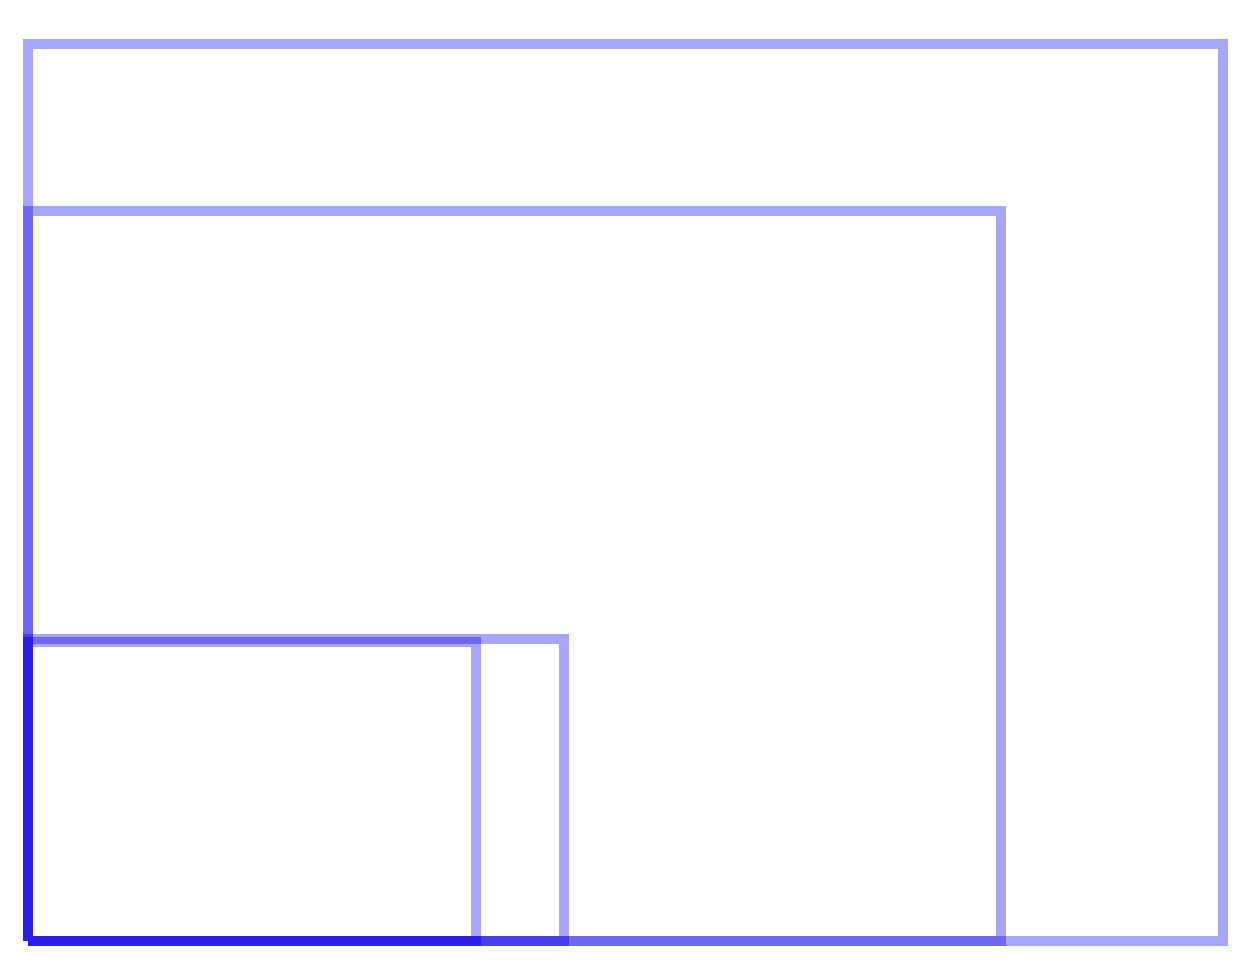
\includegraphics[width=0.98\linewidth]{./images/ios-screen.png}
  		\caption{iOS}
  		\label{fig:iOSScreenFragmentation}
	\end{subfigure}
	\caption[Screen size fragmentation of mobile devices grouped by \gls{OS}, retrieved from \cite{OpenSignal:2014aa}]{Screen size fragmentation of mobile devices grouped by \gls{OS}}
	\label{fig:MobileScreenFragmentation}
\end{figure}
\nocite{OpenSignal:2014aa}

Concluding, when creating an app for the \emph{Android} platform, the developer is facing several design decisions, which either increase the complexity of the program or reduce its functionality or accessibility. In opposite to that a developer choosing the \emph{iOS} platform can easily create an application which is optimised for all available devices, as well as exploiting all recent features offered by the \gls{OS} without excluding a big amount of users, who are not running on the latest version. 

Another decision that needs to be made is the amount of functionalities available on the different platforms. Eventually it is smarter to restrict certain functionalities to a platform or technology. This might decrease the complexity of a single application, but increase the development complexity.

In opposite of creating an application that includes all functionalities offered by the system there might be a dedicated application for administrative tasks and member related tasks. This would reduce the complexity of the respective app and hide uninteresting features from the regular user, while only creating a minor overhead for the small group of administrators. Since the tasks might be very different, even the adoption of a different platform or technology could be considered. 

\section{Architecture} % Mapping to deployment model/ER model/architectural overview
\label{sec:Architecture}
The architectural decision highly depends on the platform and technology chosen. When making this decision, it comes to choose between a multi-tier, also known as client-server, and a single-tier, also known as client-only, architecture.

In comparison to a multi-tier web application that is accessed by multiple users at the same time, the complexity of a single tier desktop application is reduced. Inevitable this comes with several negative implications. The biggest impact for an administrator is the missing possibility to delegate certain tasks to other members. On top of that locally stored information can not be accessed by any user, because of availability and security limitations of a personal computer.

\begin{figure}[h]
  	\centering
  	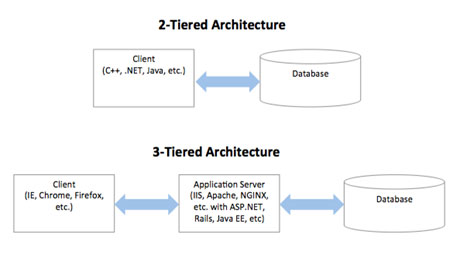
\includegraphics[width=0.7\linewidth]{./images/tier-architecture.jpg}
  	\caption[2-tier and 3-tier architecture, retrieved from \cite{Wright:2015aa}]{2-tier and 3-tier architecture}
	\label{fig:TierArchitecture}
\end{figure}
\nocite{Wright:2015aa}

In opposite to that, a multi-tier architecture enables the user to access and modify data through a centralised data provider. As shown in figure \vref{fig:TierArchitecture}, within a 2-tier architecture, the data is directly available, where a 3-tier architecture adds another abstraction or presentation layer between the raw data and the user. The decision, which kind of architecture to choose, highly depends on the application itself. 

The security of a 3-tier architecture might be more sophisticated, since the logic provided by a dynamic web server offers more possibilities to define user groups and access rights, but if the policy is not well designed, this might lead to violations. Therefore a 2-tier architecture might be a better pick, since it's configuration possibilities are more basic and therefore lead to less problems \cite{Wright:2015aa}.

Costs as well as maintainability is dependent on the complexity of the architecture. The 3-tier architecture is implicitly more complex and therefore leads to a higher costs and -in general- poorer maintainability. In opposite to that, a 3-tier application offers in most cases a better performance and its usability is more satisfying, since it provides a presentation layer \cite{Wright:2015aa}.

\section{Functionality} %Mapping to final use cases

A brief wrap up and explanation of the key functionalities was given in chapter \vref{chapter:SellingPoint}. Based on these findings several distinct functionalities of the application can be derived. Because of the limited timeframe only a subset of the presented functionalities was realised within this project.

\subsection{Administrator related functionalities}

Initially the administrator should be able to represent the organisational structure of his club within the application. In general a club is hierarchical organised, containing several divisions, with an arbitrary amount of sub-divisions. This structure is highly dependent on the respective club and therefore needs to be as customisable as possible. 

As explained in chapter \vref{chapter:SellingPoint} the administrator should be able to delegate the administration as easily as possible. Concluding it should be feasible to assign second level administrators to each division, splitting up the workload into easily manageable pieces. It is important to note that the second level administrators only have restricted access and modification rights. For example, they should only be able to view personal information of users they are directly administrating.

To manage the users of the club, the administrator needs to be able to create them. Each user should be associated with one or more division. On top of that several personal information need to be stored together with the user. These might include his address, banking information or club related information like his membership number or the dates he became active, passive or resigned from the club. This structure is dependent on the data, the club needs to operate and therefore the possibility should be given to add custom fields to the profiles of user. Upon the creation of a user, he might be informed about his new account through an automated email, where he is introduced to all features of the system and is invited to start using it.

Another time consuming task of an administrator is the management and promotion of internal events. Those events should be created by any administrator, but a second-level administrator should only be able to invite users that are part of his managed divisions. Therefore the administrator cannot invite users to events that probably are not relevant to them. For administrative purposes it would be useful to receive feedback on the participation of certain events. To simplify the process, user should be invited on a division based selection, concluding the administrator does not need to pick each relevant member but only the relevant division.

The process of collecting membership fees is complicated and in comprehensive. The application could simplify and centralise the process by offering automated debit transfer from the member's bank account to the club. Therefore the application needs to interact with the club's bank account to authorise and supervise the membership fee transactions. The usage of this feature would need a high level of trust towards the application and its creator.

Besides the promotion of events, a club -in general- needs to inform the users regular about news concerning certain division or the club. Some of these information might get shared with the public in parallel which would resolve in an unnecessary overhead. Concluding, besides the implementation of a personalised news feed, the system could also offer the possibility to connect to webpage hosting frameworks, like Wordpress or Joomla and social media platforms, enabling the administrator to share information with the user's of the society as well as the public.

Additionally the application should also respect user that are not using the application, because of security concerns or their aversion towards modern technology. It is also possible that certain user do not own a system that is supported by the application. Concluding the system should support a fall back solution for these persons and offer information through standardized channels, like electronic or non-electronic mail.

Lastly the application could aggregate interesting information for the administrator and present them within a dashboard. This might include upcoming events or statics about the usage of the platform. On top of that the system could provide reminder about anniversaries or milestone birthdays of users, which would enable the club to reliable provide congratulations.

\subsection{User related functionalities}

As shown in chapter \vref{chapter:SellingPoint} two of the three presented key functionalities are user oriented. Therefore the final application is probably going to have a fairly big amount of user related functionalities.

To get rid of different messaging technologies used within the club, a centralised group chat feature should be offered. These group chats should be created automatically for each division. User that are part of the respective division should have the ability to participate within this group chats. For the sake of simplicity, a group chat should only be available for divisions where this feature is useful, therefore the administrator should be able to select divisions where this feature is not available. To reduce the amount of notification received through a group chat, the user might only be reminded about an incoming message if he is explicitly mentioned.

The application should also support the user to manage his personalised club calendar and remind him about the beginning of upcoming events. The user should only be invited to events that apply to his respective position within the club. To support the planning of these events, the user should be able to respond to the invitation. Additionally a connection between the calendar system of the application and the native system of the respective operating system could be given, by using a standardised technology, like \emph{iCal}.

It is a difficult task for an club administrator to maintain the complete records of every user, especially if the user's contact detail change frequently. Therefore it would be a good way to delegate this task to the users. By enabling the user to update their profile on their own, the process is simplified for the administrator and the user. It also enables the user to give his appearance a personal touch, which might be discoverable by other users, if the permission was given.

The application could also provide a counterpart for the news published by administrators. This centralised newsfeed could provide user tailored information about relevant topics. The user could also decide about the amount and kind of notification he receives about these information. On top of that the user might be able to opt-in an email newsletter system or rss feed of the club.

Another problem, a lot of clubs are facing is the problem of collecting useful and up to date information that can be used to promote the club or events on their webpage, in the newspaper or internally. The system could enable every user to hand in articles written about recent activities or to upload pictures and videos that are club related. These information should only be published if they are approved by an administrator, or handed in by a trusted user.

\section{User Interface} %% Mapping to wireframes

As discussed in chapter \vref{sec:UserAnalysis}, one of the most crucial parts of a system is the user interface, since this is the only part of the system the user is directly interacting with. Concluding a bad designed user interface can increase the complexity of an application as well as decrease user satisfaction 

The design concepts for an administrator focused web application and a user focused iOS application are presented in the following sections. In general the navigation concept is a crucial piece of these application. A very popular option to manage the navigation on webpages and mobile application is the so called \enquote{Hamburger Menu} \cite{Abreu:2014aa}. The three parallel horizontal lines indicating that there are more options available are widely used. Unfortunately there are several problems with this concept, including but not limited to lower discoverability, less efficiency, a clash with platform navigation concepts and the inability to get a glance view on the available options \cite{Abreu:2014aa}.

\subsection{Web application}

In general a web application has the possibility to display its information either horizontal or vertical. A combination through dropdown boxes is possible but should be avoided, because of the lower discoverability and less efficiency, already discussed above. \cite{Crestodina:2015aa}

On top of that it is important to put only a small amount of items in the navigation bar. This is based on the fact that the human short term memory in general is only able to hold an average of 7 items, and therefore the user would start forgetting items at the top of the list while scanning through the available navigation items. When limiting the amount to 5 items this would increase the importance of the remaining items, while increasing simplicity of the webpage itself. \cite{Crestodina:2015aa}. 

Psychology studies have shown that the most important items within a list are the first and last ones. Therefore a designer should consider the placement of important navigation items either at the beginning or end of the list. \cite{Crestodina:2015aa}

It is important to note that a user faster adopts well known structures and navigation concepts. Therefore using a non-standard navigation concept could decrease the usability even if it would solve problems of existing solutions, just because of the fact, that the user is not used to it. Especially when placing the navigation items in an unfamiliar place could lead to confusion. \cite{Crestodina:2015aa}

To increase usability, the user should always be aware of his current position within the application. On top of that the user should be given the possibility to change his current position at any time. This requires the need of always visible navigation elements. 

While all of this holds true in general the exceptions of these rules, are the concepts that a user is going to remember later. Although creating a new navigation concept, which is respecting only a subset of the above stated suggestions, or none of them, requires a lot of conceptional work. Besides that, the implementation of a non-standardised system also requires the need of starting from the scratch, which increases the workload drastically. \cite{Hampton-Smith:2013aa}

Besides the consideration of different navigation concepts the overall design of the different functionalities were also considered. However for the sake of simplicity only their final designs are presented in chapter \vref{sec:Wireframes} and \vref{sec:GUI}. Especially since the formal definition of all functionalities, that are going to be implemented within this project, has not been given yet, this list would exceed the scope of this paper.

\subsection{iOS application}
\subsubsection{Navigation}
When creating an iOS application, a lot of design elements are pre-defined by the \gls{OS}. On the one hand this leads to well known design and navigation principles and following the guidelines will -in general- lead to a well designed application. On the other hand the applications are not very distinguishable based on their design and might become boring for the user. Concluding using an adjusted layout or navigation concept might lead to a better recognisability of the brand. 

\begin{figure}[h]
  	\centering
  	\includegraphics[width=0.8\linewidth]{./images/ui-concept.jpg}
  	\caption[Early navigation concept drawing (own figure)]{Early navigation concept drawing}
	\label{fig:NavConcept}
\end{figure}

Figure \vref{fig:NavConcept} shows early design concept drawings. On the left, a standard tab bar concept is presented. The bar contains a total of five elements, including \emph{Messages}, \emph{News}, \emph{Photos}, \emph{Events} and \emph{Settings}. This design is an example of a predefined layout provided by \emph{Apple}. It is important to note that there is no default design that uses the \enquote{Hamburger menu} described above. The tab bar is therefore a viable alternative, which would fit into the design-system of \emph{iOS} and consequentially might perish between the millions of other available application. Nevertheless very popular companies use this concept with minor adjustments, including \emph{Facebook}, \emph{Yelp} and \emph{Twitter}.

In opposite to that the left side of figure \vref{fig:NavConcept} describes a very different navigation concept. The author did not find this concept in any other application, although it was inspired by \emph{Todo Movie}'s sharing layout, as well as \emph{Google}'s material design. The main idea is the positioning of a fixed menu button in the lower part of the screen. When pressing this visual element, one of the two frames shown in the middle of figure \vref{fig:NavConcept}, would appear, revealing the menu. It might either be a \enquote{Navigation Wheel}, that could be operated using swipe gestures, or the available items could appear by moving up.

This concept has several advantages and disadvantages. By choosing a full screen presentation of the menu items, the amount of elements could be increased from a maximum of five, when using a tab bar, to about seven. This is the suggested maximum of navigation items, since the average person has a short term memory of seven elements \cite{Crestodina:2015aa}. On top of that, most of the user prefer well designed swipe gestures over taps, which might be adopted using the \enquote{Navigation wheel} menu. Since the menu button is a fixed item on top of most of the screens, this would attract the attention of the user and improve the engagement. On the opposite, this concept has similar downsides as the previously presented \emph{Hamburger menu}, which is, amongst others, missing the possibility to glance the available items \cite{Abreu:2014aa}.

\subsubsection{Chat overview}
For the sake of simplicity only the layout of the chat overview page is going to be discussed besides the navigation concept. Figure \vref{fig:ChatScreens} shows these screens of the two most established chat applications on the \emph{iPhone}, \emph{WhatsApp} and \emph{iMessage}. Obviously both concepts are very similar, since they both use a table view with slightly different cell layouts. This kind of concept is very useful, when there is the need of showing a big amount of items in an precise and easy to retrievable way. 

\begin{figure}[h]
	\centering
	\begin{subfigure}{.33\textwidth}
  		\centering
  		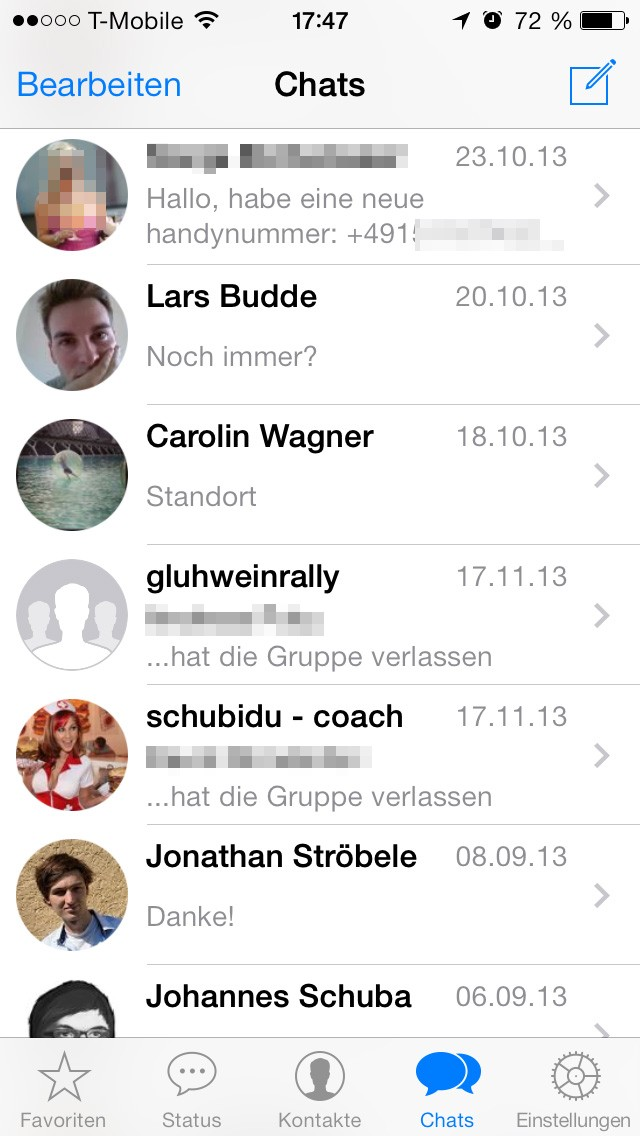
\includegraphics[width=0.98\linewidth]{./images/whatsapp-screen.jpg}
  		\caption{WhatsApp}
  		\label{fig:ChatWA}
	\end{subfigure}
	\begin{subfigure}{.66\textwidth}
  		\centering
  		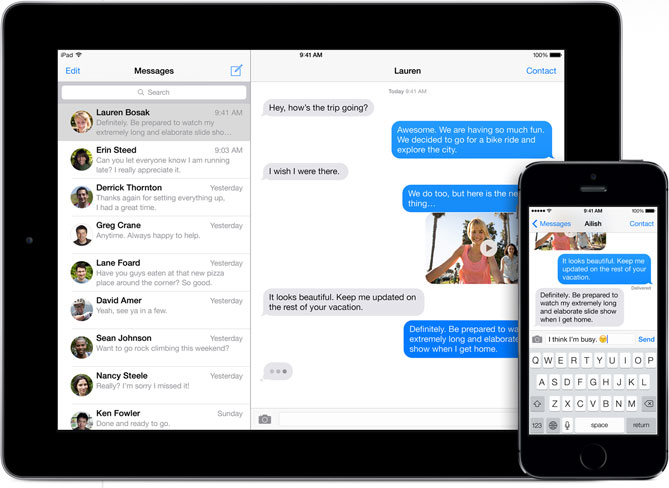
\includegraphics[width=0.98\linewidth]{./images/imessage-screen.jpg}
  		\caption{iMessage}
  		\label{fig:ChatiMessage}
	\end{subfigure}
	\caption[Chat overview screen shots of established messaging apps retrieved from \cite{Inc.:2015aa} and \cite{Stuckler:2013aa}]{Chat overview screen shots of established messaging apps}
	\label{fig:ChatScreens}
\end{figure}
\nocite{Inc.:2015aa, Stuckler:2013aa}

Nevertheless the amount of available chats within \emph{myVerein} is very likely being limited to a foreseeable small quantity. Therefore, other concepts, besides the established list might be considered to increase the uniqueness and recognisability as well as usability. The proposed concept includes two circles per row with a caption, each representing an available chat. The chat with the latest message would be shown on the top left of the screen. Every chat bubble would have a caption stating the name of the division, whose chat it is representing. The image of the bubble would show the image representing the user, who sent the latest message. This might help the user to estimate the importance of the message. A \enquote{tap-and-hold} feature could also be included, showing a preview of the last couple of messages without entering the chat.

\subsubsection{App icon}
Maybe one of the most important visual items of a mobile application is its icon. It needs to be well designed, since the users are going to put it on his home screen and probably see it every day. On top of that it needs to be interesting enough to regularly click on it, but not too distractive. Lastly and most importantly the user needs to be able to look at the app icon and directly associated it with the product. \cite{Flarup:2015aa}

As shortly covered above it is essential to keep some things in mind when working on a good app icon for mobile phones. The first thing to note is scalability. When developing an application for \emph{iOS 8} a developer has to bundle 12 different resolution for the application icon and it has to look good in every one. Concluding \enquote{[o]verly complicated icons that try to cram too much onto the canvas often fall victim to bad scalability} \cite{Flarup:2015aa}, therefore the designer should embrace simplicity and check that the icon looks good on top of different background colours. \cite{Flarup:2015aa}

\begin{figure}[h]
  	\centering
  	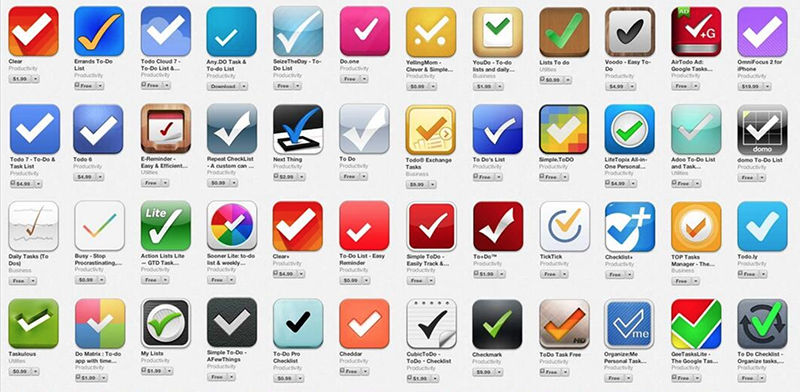
\includegraphics[width=0.7\linewidth]{./images/productivity-icons.png}
  	\caption[App-Icon design within the productivity category, retrieved from \cite{Flarup:2015aa}]{App-Icon design within the productivity category}
	\label{fig:AppProd}
\end{figure}
\nocite{Flarup:2015aa}

While keeping the icon scalable it is important to create a design that is recognisable. Therefore the app should not be overcomplicated. When trying to create such an icon it is useful to observe competitors in the same field as well as other popular app icon designs. \cite{Flarup:2015aa}

When looking at the competitor's app icons, it is important to note that a developer should not copy there design. Because uniqueness is another very important aspect of the icon layout, since it needs to attract the attention of the user, and should stand out of the competition. A negative example is the productivity category on the app store, shown in figure \vref{fig:AppProd}. Since all of the shown apps trying to solve a similar problem, they all end up having a more or less identical icon. When ending up, choosing a single glyph, like a checkmark, the designer needs to to make a difference by using a rich colour design. \cite{Flarup:2015aa}

Last but not least it is crucial to avoid text within an app icon. On the one hand, this text scales very badly, on the other hand the app is always accompanied with a caption, stating its name. Consequently a logo should not be used as an icon, since these two are very distinct \cite{Flarup:2015ab}. Nevertheless a single letter, used for example by the \emph{Facebook} app, might be a good way to create a distinguishable brand.

\begin{figure}[h]
  	\centering
  	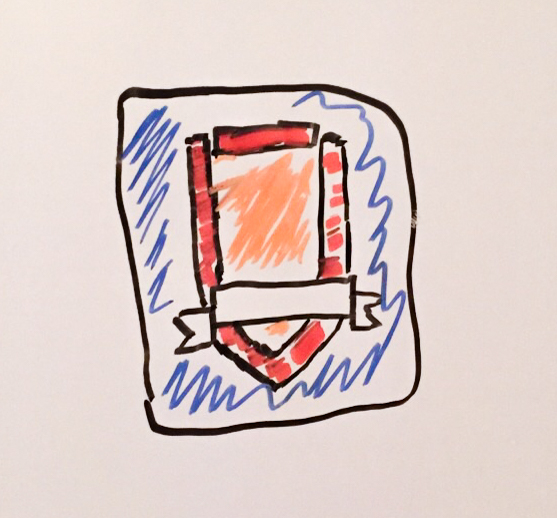
\includegraphics[width=0.5\linewidth]{./images/app-sketch.jpg}
  	\caption[Early application icon sketch (own figure)]{Early application icon sketch}
	\label{fig:AppSketch}
\end{figure}

After considering all of the above stated concerns and doing some brainstorming, the best suitable association and unique association with a club, that was found, was an emblem. Figure \vref{fig:AppSketch} is showing an early sketched, created during this session. This very generic object is widely used as a foundation for many logos of different clubs. By leaving the banner empty, it leaves space for the user to imagine his club name or description into it. 

It was considered to form the emblem in a way to resemble to letter \enquote{V}. This could have let to an association with the application's name \emph{myVerein}, similar to the \emph{Facebook} logo. 

\subsection{Colour scheme}

Within the last sections we only looked at the different geometric aspects that can be altered within the application to change the visual appearance. Within this section another very important part of the \gls{UI} is considered: The colours used to tint the visual elements. 

The field of colour theory is a very complex one, therefore the time only permitted a very basic analysis on this specific matter. The first thing to note is that different colours have different very distinct meanings. In general a slight change in saturation might lead to a completely new impression of a colour \cite{Chapman:2010aa}. For example the colour red is considered as a violent or aggressive colour, while green is more balancing, relaxing and down to earth \cite{Chapman:2010aa}.

After choosing an appropriate base colour, it is important to create a colour palette, since a single colour would make the application boring, and the developer would be unable to highlight certain entries using a different tint. There are several techniques to create a colour pattern. When using a \emph{Monochromatic} colour scheme the base colour is only altered using different tones, shades and tints \cite{Chapman:2010ab}. 

\begin{figure}[h]
  	\centering
  	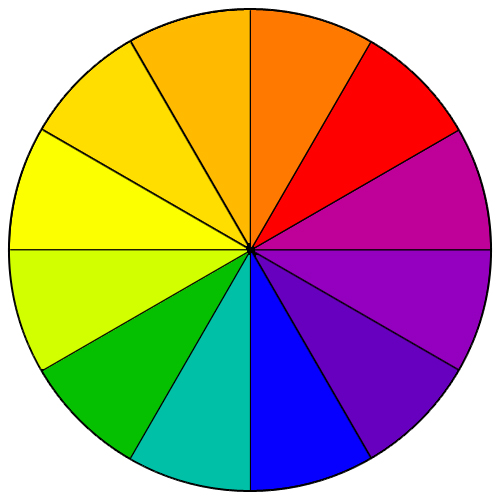
\includegraphics[width=0.5\linewidth]{./images/colorwheel.jpg}
  	\caption[12-spoke colour wheel, retrieved from \cite{Chapman:2010ab}]{12-spoke colour wheel}
	\label{fig:ColourWheel}
\end{figure}

Figure \vref{fig:ColourWheel} is showing a 12-spoke colour wheel, which is used when creating an \emph{Analogous} colour scheme. It is created by picking three colours that are next to each other and adjust their tones, shades and tints, just like the \emph{Monochromatic} colour scheme would do it \cite{Chapman:2010ab}. This scheme is creating a set of colours, that are very close to each other.

Since the \emph{Analogous} colour scheme is sometimes regarded as being boring, since the colours are very similar, the \emph{Complementary} scheme introduces a wider range, by selecting the colour opposite of the base within the colour wheel \cite{Chapman:2010ab}. This one is most likely being very different to the base colour and adds depth to the palette.

The most diverse colour scheme is called \emph{Tetradic} or \emph{Double-Complementary}. It is regarded as the most difficult scheme when trying to create an efficient palette \cite{Chapman:2010ab}. The scheme is \enquote{based on the tetrade — the foursome of colors evenly distributed on the fourths of the color wheel} \cite{Stanicek:2011aa}. Since this scheme is considered more nervous than the other ones \cite{Stanicek:2011aa}, the primary colour should be used for the main design, while the others are only sparely used for accents \cite{Chapman:2010ab}.

\chapter{Design}

Using the initial thoughts and concept alternatives presented in chapter \vref{chapter:Concept} a design is going to be developed within this chapter. Based on this design the final implementation of the project is executed.

The author of this paper decided to implement the system using a three tier architecture (see section \vref{sec:Architecture}) using a user facing mobile iOS app and an administrator facing web application (see section \vref{sec:Platform}. The remaining details are discussed below.

\section{Requirements}
\label{sec:Requirements}
The software requirement specification \cite{Steiler:2014aa} and in more details the server requirement specification \cite{Steiler:2014ab} state the formal requirements of the product. The requirements are separated in obligatory, optional and additional requirements as well as isolating several functionalities within the non-requirements. The basic requirements on the application are presented in the following, respecting the thoughts and findings from the earlier chapters.

\subsection{Obligatory requirements} % must-have
The fulfilment of the following criteria is mandatory:

\paragraph{User}
\begin{itemize}
\item The user needs to be able to log himself into the server provided by his club at the start of the application
\item The user needs to be able to check the upcoming schedule of the club
\item The user needs to be able to send and receive messages
\end{itemize}

\paragraph{Administrator}
\begin{itemize}
\item The administrator needs to be able to modify the server according to the clubs name etc. during the initial setup
\item The administrator needs to be able to modify the access rights of all members of the club
\item The administrator needs to be able to schedule an event
\item The system needs to ensure a fault tolerant, consistent operation.
\item The system needs to be configurable
\item The system needs to provide a secure user authentication
\item The system needs to handle the login of multiple users at the same time
\item The system needs to handle several messages at the same time
\item The system should be configurable through a web interface, that enables the administrator to manage user
\item The system needs to operate according to the data privacy act
\item The system needs to be designed in a way that a user can only access a minimum amount of private data of the other users
\item The system needs to be designed to be easily extensible
\item The system needs to save and gather the data from a persistent data storage system
\item The system needs to be developed in Java 8
\end{itemize}

\paragraph{Application (Client)}
\begin{itemize}
\item The application needs to be optimised for the operation with an iPhone 6
\item The application needs to ensure an intuitive operation
\item The application needs to have a logic menu structure
\item The application needs a basic graphical user interface
\end{itemize}

\paragraph{System (Server)}
\begin{itemize}
\item The system needs to ensure a fault tolerant, consistent operation.
\item The system needs to be configurable
\item The system needs to provide a secure user authentication
\item The system needs to handle the login of multiple users at the same time
\item The system needs to handle several messages at the same time
\item The system should be configurable through a web interface, that enables the administrator to manage user
\item The system needs to operate according to the data privacy act
\item The system needs to be designed in a way that a user can only access a minimum amount of private data of the other users
\item The system needs to be designed to be easily extensible
\item The system needs to gather the data from a relational database
\item The system needs to be developed in Java 8
\end{itemize}

\subsection{Optional requirements} % nice-to-have
The following requirements are optional, but their implementation is nice to have.
\begin{itemize}
\item The application should have a sophisticated graphical user interface through a web interface
\item The administrator should be able to create divisions
\item Each user should be able to be part of one or more divisions, to only receive relevant information.
\item The system should support private chats for each division
\item Invitations to events should be send to divisions
\item The user should be able to request access to a division, this access is granted by a higher level user
\item The user should be able to share photos that are relevant to the club
\item The application should use push notifications to effectively alert the user about incoming messages, news or upcoming events
\item The system should be designed to ensure extensibility
\item The user should be able to optional create a public profile containing contact information
\item The system should be designed to allow a multi-lingual implementation
\item The administrator should be able to manage the divisional arrangement via the web interface
\item The mobile application should be developed using Swift
\item The mobile application should be created according to the Apple Developer Guidelines
\end{itemize}

\subsection{Additional requirements}
The following requirements would improve the overall user experience, but their implementation is not business critical.
\begin{itemize}

\item The application could have a central news feed, which contains the latest information provided by the administrator
\item The administrator could be able to publish relevant information through the web interface
\item Approved user besides the administrator could be able to manage user or publish news and events
\item The system could send an Email newsletter for members that are not owning a smartphone running iOS, or allow the print out of the newsletter for a non-digital distribution
\item The events could support assignment of supporting roles needed during the event
\item The events could support voting buttons to find the ideal date for the meeting
\item The system could support the download of shared pictures
\item The system could support the use of shared pictures within the news of the club
\item The system could allow the administrator to share news through the clubs homepage using plugins within Joomla, Wordpress, Facebook or other systems.
\item The application could be implemented bilingual (English, German)
\item The system could have a second member type, that is allowed to publish news and events
\item The application could be able to send and receive attachments in messages, like photos or audio messages
\item The application could handle multiple accounts on different or on the same server
\item The application could support the native resolution of different devices, like the iPad or the iPad mini
\item The system could support the use of shared pictures within the news of the club
\end{itemize}

\subsection{Non-requirements} %need-not-to-have
The following requirements are not in the scope of this product.
\begin{itemize}
\item The system is not designed to create a homepage for the club
\item The application is not designed to provide access to non-members of a club
\item The application is not designed to work without a server where the user is able to authenticate himself
\item The system should not be used to collect statistics about the users
\end{itemize}

\section{Use cases}
%Within this section the  use cases derived from the requirements defined in 
To be added...









\section{Architectural model}
After reviewing the findings in section \vref{sec:Architecture} and considering the requirements in section \vref{sec:Requirements} the decision was made to use a 3-tier architecture, based on the possibility of a more sophisticated security policy and an advanced business logic. The design was created, keeping scalability in mind. Figure \vref{fig:Architecture} shows the planned architecture of the system. 

\begin{figure}[h]
  	\centering
  	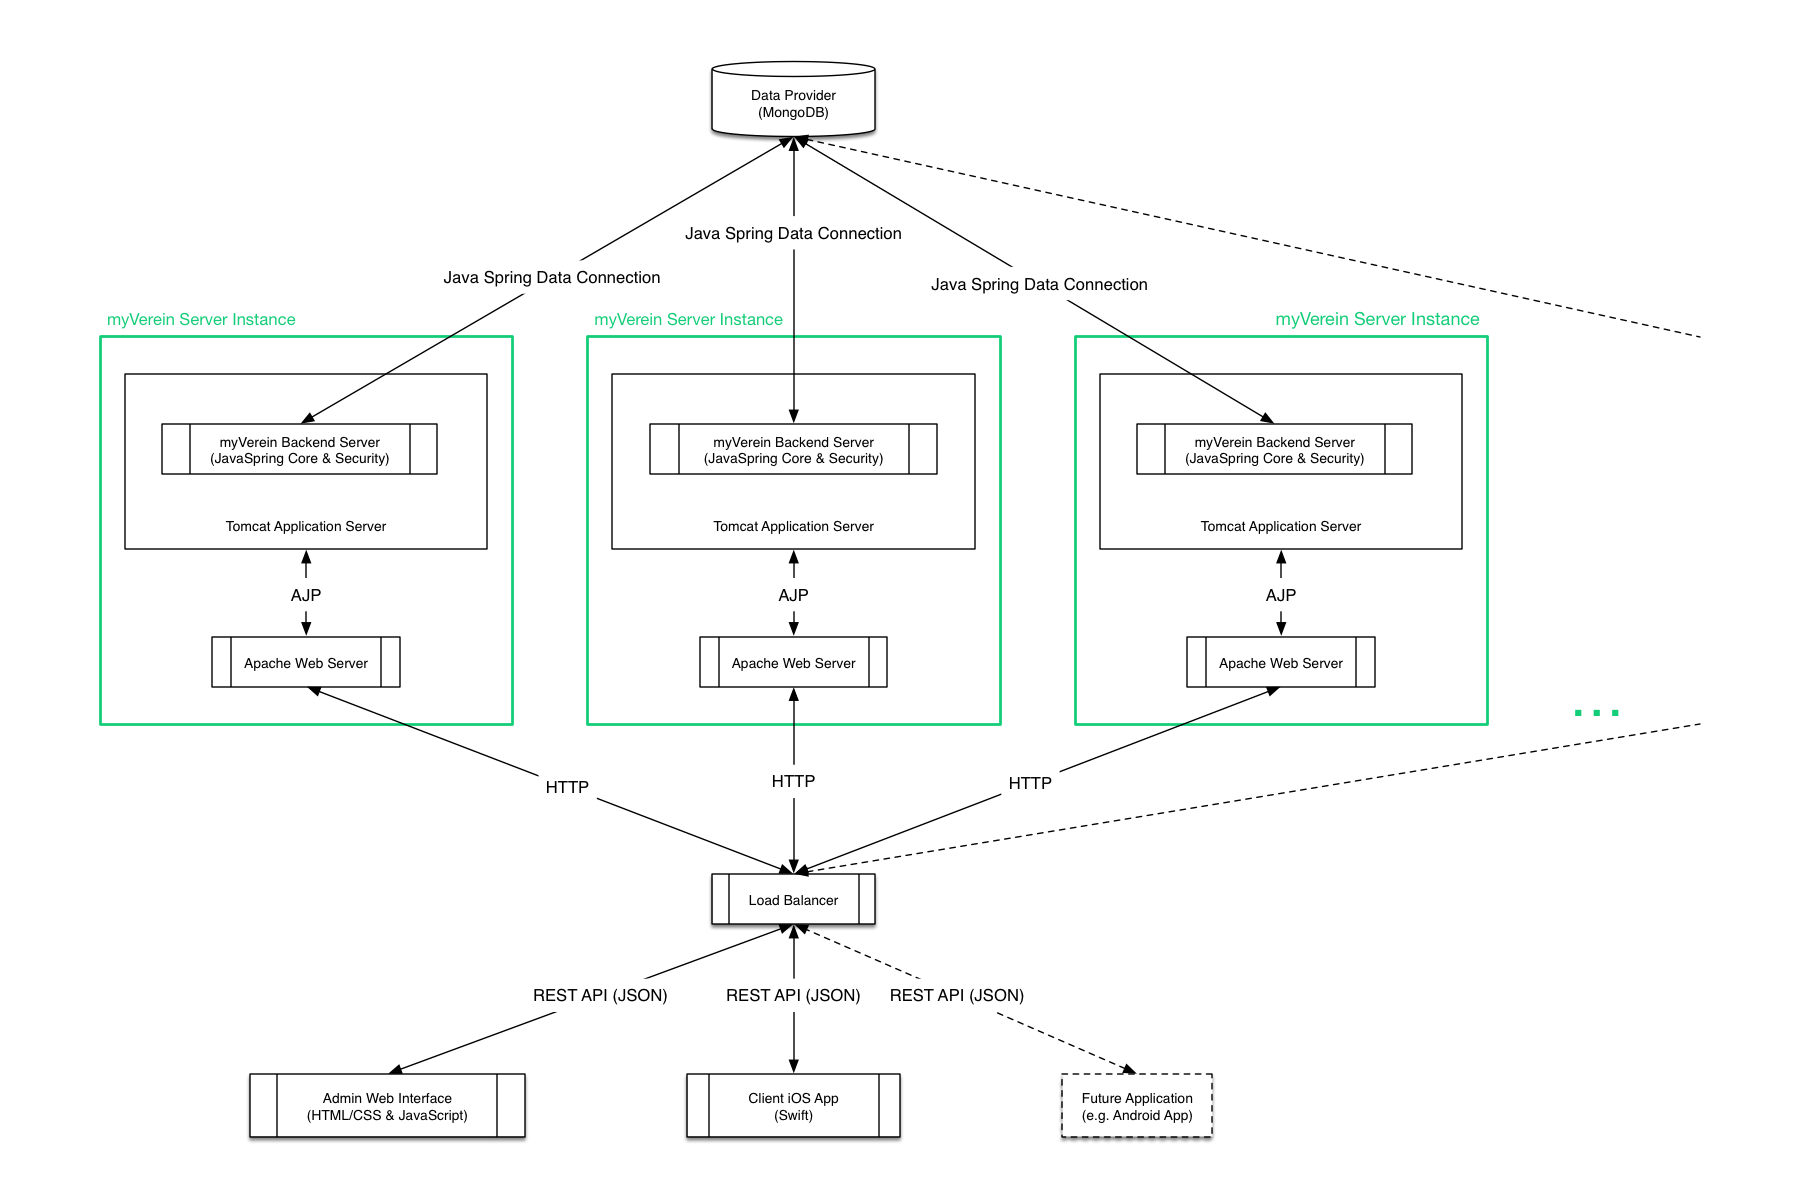
\includegraphics[width=0.95\linewidth]{./images/architecture.png}
  	\caption[System architecture (own figure)]{System architecture}
	\label{fig:Architecture}
\end{figure}

The central server software is written in \emph{Java 8} and uses the \emph{Java Spring} framework. This mature open source framework provides sophisticate security configurations as well as several access frameworks for data provider. On top of this platform several other additional frameworks are available, including messaging and social media connection, that can be used to easily extent the functionalities of the application. The complete business logic is implemented on top of this framework.

Since the server application needs to be run within the \gls{JVM} and be able to communicate with other machines, an application server is neccessary. For this test environment a \emph{Tomcat 8} application server was chosen to host the application. For the possibility to easily and efficient server static content, the application server is connected to an Apache web server using the \gls{AJP}. 

The data provider was chosen to be a \emph{MongoDB} \gls{NoSQL} database system. This schema free database enables flexibility, as well as extensibility and speed, which is not comparable to existing relational database applications \cite{Moschetti:2014aa}. The database itself is connected with the server application using the \emph{Spring Data} framework, which supports the use of \emph{MongoDB}. This framework provides a concise and object oriented access to the database using the native \emph{Java} driver developed by \emph{MongoDB}. Most importantly it integrates very well into the \emph{Java Spring} framework.

To ensure high flexibility the system is designed to operate behind a load balancer. Therefore each system needs to be stateless and retrieve all necessary information and configuration from the central data provider. If this is the case, the necessary computing power to fulfil all requests can be automatically allocated and deallocated, by deploying additional \emph{myVerein Server Instances}, or removing them. This would allow a cost efficient, high available, large scale operation within a cloud environment.  

The front end of the system consists of an iOS app and a web application. Both of them use a \gls{REST} \gls{API} to communicate with the system. The \gls{API} is designed to be used by many different application and should therefore simplify the process of adding new front-end components to the system. By using this model, the development of these components can be done independently from the development of the server as long as the existing \gls{API} is not changed.

The web application is intended to be used by the administrator only to manage the system. Within this web application only the features that are relevant for the administrator need to be accessible. This application should avoid the reloading of the current page by using the principles of \gls{AJAX}. On top of that the application should be designed to be as mobile friendly as possible, to enable administrators to use it on their mobile devices as well. To create a rich \gls{UI} and feature set, while keeping the workload on the developer as small as possible, several \gls{CSS} and \gls{JS} frameworks are going to be used.

The iOS application's target group are the member's of the clubs using this system. The application is going to be developed using \emph{Apple}'s new programming language \gls{SWIFT}. Additionally the dependency manager \emph{CocoaPods} is going to be used for adding existing frameworks to the project. This is done to simplify the development of the application, while increasing the usability.

\section{Database layout}

As presented in section \vref{sec:Architecture} the data provider used for this project is going to be the \gls{NoSQL} database system \emph{MongoDB}. Even though this system uses a dynamic schema, it is important to model the organisation of the data in advance, to later ensure a reliant and consistent operation. Nevertheless this schema is very likely going to change during development, but the dynamic aspect is very helpful within the context of this agile development approach.

A database schema can be depicted using an \gls{ER} diagram. This visual representation of a database layout was originally introduced for relational databases, nevertheless it was adopted for this work into the context of \gls{NoSQL} databases. The diagram created during the design phase and used as orientation during the development can be found in appendix \vref{app:ERDesignPhase}. It is important to note, that during the design of the database schema all requirements discussed in \vref{sec:Requirements} have been considered.

Within this sections each entity, in the context of a document oriented database like \emph{MongoDB} better known as document store, is going to be described in details. The connection between documents is also discussed.

\subsection{User}
The user information are stored within the \emph{User} document store. The data is organised according to the \emph{One-to-Many Relationships with Embedded Documents} model \cite[p. 141]{Mongo:2014aa}.

On the lowest level all required information about the user, like the user's email or his hashed password, are stored. The private information of a user, which can only be viewed by the administrator are saved within the \emph{PrivateInformation} array. The \emph{PublicInformation} array is holding all optional information stated by the user. These information can be accessed by every member of the club.

On top of that each user is part of one ore more divisions. The membership within the divisions is stored as nested arrays. These data structures hold the foreign key to the division as well as the date when the user joined the division.

\subsection{Division}
Each division is an entry within the division's document store. It is defined by its name and short description.

Divisions are organised hierarchical within a club, so this structure has to be represented within the database. This data structure is going to be represented within MongoDB using the \emph{Model Tree Structures with an Array of Ancestors} \cite[p. 149]{Mongo:2014aa}. This structure is storing the direct parent of the node, as well as an array of all ancestors, to easily query all ancestors. Within the use case of this application this behaviour is needed, since the system needs to subscribe the user to all chats of the user's division as well as all chats above his division.

Each division is administrated by up to one user, who gains access to the administrator panel through this position. If there is no administrator specified, the super admin takes his role. This super user is defined by being administrator of the root division.

\subsection{Messages}
Each member of a division automatically joins a group chat between all members of this division. To ensure privacy for each chat, messages are only saved on the server as long as necessary. Therefore a \emph{Message stack} document store is created. Every sent message is stored there until the recipient accesses it, or the system deletes the message after its expiration. The expiration of the message is handled by MongoDB through the functionality to set a Time-To-Life for collections \cite[p. 198]{Mongo:2014aa}.

Each entry contains the message to one member of the group chat. When the user syncs his application with the server, the server returns all messages from the stack for the user. The rows are deleted as soon as the user receives the message. 

\subsection{Events}
A core feature of the application is the creation and management of events for each division. The events are managed within the \emph{Event} data store. An event invites whole divisions, and every member can send a response to the invitation. 

The invited divisions are stored as embedded documents according to the \emph{One-to-Many Relationships with Embedded Documents} model \cite[p. 141]{Mongo:2014aa}, because it is unlikely that the user is going to add values to that field. If the amount of data added to these fields extends the reserved space for the document, the database has to reallocate the space, which leads to fragmentation and a slow write performance. Concluding the responses of the users is stored according to the \emph{One-to-Many Relationships with Document References} model \cite[p. 143]{Mongo:2014aa}, since these fields are constantly extended.

The database is trying to keep the used storage low and therefore tries to delete all events that have already passed. Besides that the event has several properties, e.g. a short description, a location, the date of the event and its last change.

\subsection{Pictures}
Since the user is able to upload pictures that are relevant to the club, a document store is created to manage these pictures. The picture's metadata is handled through that store, as well as the URL pointing to the file and an array with tags for the picture.

Each picture is uploaded by a specific user and the user can associate up to one division to the picture.

\section{Wireframes}
\label{sec:Wireframes}

\section{Licensing}

\chapter{Implementation}
Umsetzung (Wie sieht es am ende aus, besonderheiten, tests aus entwurf -> Def aus pflichtenheft)

\section{Backend}
\subsection{Database}
\subsection{Business logic}

\section{Front-end}
\subsection{Web-Application}
\subsection{iOS Application}

\section{Logo and colour scheme}
\label{sec:GUI}
color, logo, GUI

\chapter{Ongoing work}
\label{chapter:OngoingWork}
ausblick (max 1/8 vom text)

